\documentclass[11pt,a4paper]{article}
\usepackage[utf8]{inputenc}
\DeclareUnicodeCharacter{2248}{\ensuremath{\approx}}
\usepackage[T1]{fontenc}
\usepackage[brazil]{babel}
\usepackage{lmodern}
\usepackage[margin=2cm]{geometry}
\usepackage{amsmath,amssymb,bm}
\usepackage{graphicx,booktabs,float,longtable,url}
\usepackage{xcolor}
\definecolor{azul}{RGB}{0,70,200}
\definecolor{verm}{RGB}{200,0,0}
\usepackage[hidelinks]{hyperref}
\title{Confiabilidade de taludes com campos aleatórios no NeoPZ\\\large Relatório parcial: plano de trabalho, formulações,
testes, hipóteses e o mapa dos relatórios}
\date{17/11/2026}
\begin{document}
\maketitle
\tableofcontents

\section{Objetivo e onde estamos}
O trabalho serve a dois artigos:
\begin{itemize}
  \item \textbf{Amostragem por importância (AI)} para taludes com campos aleatórios no MEF. A validação é no Ceron (2025),
    no rebaixamento, e no Cho (2010), um talude seco com $c'$ e $\varphi'$ como campos correlacionados e $P_f$ de 0,4\,\% a
    2\,\%.
  \item \textbf{Chuva em talude não saturado} (Rahardjo et al., 2007), com as mesmas ferramentas: Monte Carlo, FORM e AI.
\end{itemize}
O plano de trabalho (\path{Projects/PlanoDeTrabalho/README.md}) valida as ferramentas uma de cada vez, antes de usá-las
na chuva. As etapas 0 a 3 estão rodadas, e a 2c (gradiente modal) foi testada no PC. A etapa 4 (FORM e AI na chuva) tem
a referência pronta, e a etapa 5 (a investigação da chuva) ainda não começou. Tudo roda no cluster fermi (4 nós, 48
processos); o PC serve para testes curtos. Este relatório reúne o que está espalhado em vários documentos (Seção~\ref{sec:mapa}).

\section{Formulações}
\subsection{O modelo mecânico e o fator de segurança}
\begin{itemize}
  \item \textbf{Material:} Mohr--Coulomb elastoplástico com fluxo associado, dentro do material não saturado
    \texttt{TPZMatUnsaturatedUPwPa} ($u$--$p_w$--$p_a$; \path{docs/biot_nao_saturado}, \path{formulacao.pdf}). No talude
    seco, as pressões ficam congeladas em zero.
  \item \textbf{FS pelo SRM:} $c'/F$ e $\tan\varphi'/F$ até o colapso, com arc-length no parâmetro $F$ e refinamento
    adaptativo em $h$ (tri2 + 4 níveis; \path{docs/fs_arc_length}). Esse FS é o do equilíbrio limite (Ceron 2025, Eq.~58).
  \item \textbf{Correção do SRM (etapa 1):} o peso é aplicado com $F_0 = 0{,}8$, e não com 1. Com 1, o peso às vezes
    convergia num talude com FS logo abaixo de 1, e o FS saía $\ge 1$, o que deixava um buraco no histograma.
\end{itemize}

\subsection{Campos aleatórios: as duas bases de Karhunen--Loève}\label{sec:kl}
Os parâmetros de resistência são campos lognormais, com correlação cruzada $\rho = r(c, \varphi)$ entre os campos
gaussianos:
\begin{equation}
  \ln c'(\bm x) = \mu_c + \sigma_c Z_c(\bm x), \qquad
  \ln\varphi'(\bm x) = \mu_\varphi + \sigma_\varphi\big[\rho\, Z_c(\bm x) + \sqrt{1-\rho^2}\, Z_\varphi(\bm x)\big],
\end{equation}
com $\sigma^2 = \ln(1 + \mathrm{CoV}^2)$ e $\mu = \ln m - \sigma^2/2$ (médias $m$ de 10\,kPa e 30$^\circ$, CoV de 0,3 e
0,2). $Z_c$ e $Z_\varphi$ são campos gaussianos padrão independentes, com a covariância exponencial separável
$C(\bm x, \bm x') = \exp(-|x - x'|/l_h - |y - y'|/l_v)$, $l_h = 20$\,m e $l_v = 2$\,m. Cada um é uma expansão de
Karhunen--Loève truncada:
\begin{equation}
  Z(\bm x) = \sum_{k=1}^{M} \psi_k(\bm x)\,\xi_k, \qquad \psi_k(\bm x) = \sqrt{\lambda_k}\, f_k(\bm x), \qquad
  \xi_k \sim N(0, 1) \text{ independentes},
  \label{eq:kl}
\end{equation}
em que $(\lambda_k, f_k)$ são os autopares da covariância num domínio $D$,
$\int_D C(\bm x, \bm x') f_k(\bm x')\,d\bm x' = \lambda_k f_k(\bm x)$, com $\int_D f_k f_l\,d\bm x = \delta_{kl}$. Uma
realização é o vetor $\bm\xi = (\bm\xi_c, \bm\xi_\varphi) \in \mathbb R^{2M}$, e a base entra só pelas funções $\psi_k$
nos pontos de integração. As duas bases diferem no domínio e no cálculo dos autopares.

\paragraph{KL analítica} (\texttt{KLSeparavel.h}, \texttt{RandomField}). $D$ é o retângulo $[0, 30]\times[0, 15]$\,m
que contém o talude. O kernel é o produto de dois kernels exponenciais 1D, então os autopares 2D são produtos dos 1D,
$f_k(x, y) = f^x_i(x - x_c)\, f^y_j(y - y_c)$ e $\lambda_k = \lambda^x_i \lambda^y_j$, em ordem decrescente de
$\lambda$ ($x_c$, $y_c$: o centro do retângulo). Para o kernel $e^{-|s - t|/L}$ em $[-a, a]$, com $c = 1/L$, os
autopares têm forma fechada (Ghanem e Spanos, 1991):
\begin{equation*}
  f(s) = \frac{\cos\omega s}{\sqrt{a + \frac{\sin 2\omega a}{2\omega}}}, \ \ \omega\tan\omega a = c; \qquad
  f(s) = \frac{\sin\omega s}{\sqrt{a - \frac{\sin 2\omega a}{2\omega}}}, \ \ \omega + c\tan\omega a = 0; \qquad
  \lambda = \frac{2c}{\omega^2 + c^2}.
\end{equation*}
Com $M = 2000$, a variância retida é 0,988 (média no retângulo). Parte da base descreve a região fora do talude, que não
pesa no FS: é por isso que ela precisa de mais termos.

\paragraph{KL de Nyström} (\path{Projects/Cho2010/nystrom_base.py}). $D$ é o próprio talude $\Omega$. A quadratura do
ponto médio numa grade de $0{,}5\times0{,}25$\,m dá $n = 2400$ nós $\bm x_j$, com pesos $w_j$ (a área da célula), e a
equação integral vira um problema de autovalores simétrico:
\begin{equation*}
  W^{1/2} C W^{1/2}\,\bm v_k = \lambda_k\,\bm v_k, \qquad C_{ij} = C(\bm x_i, \bm x_j), \qquad
  f_k(\bm x_j) = v_{kj}/\sqrt{w_j}, \qquad \textstyle\sum_j w_j f_k(\bm x_j) f_l(\bm x_j) = \delta_{kl}.
\end{equation*}
Fora dos nós, a fórmula de Nyström interpola a autofunção pelo próprio kernel:
\begin{equation}
  f_k(\bm x) = \frac{1}{\lambda_k}\sum_{j=1}^{n} w_j\, C(\bm x, \bm x_j)\, f_k(\bm x_j), \qquad
  \psi_k(\bm x) = \frac{1}{\sqrt{\lambda_k}}\sum_{j=1}^{n} w_j\, C(\bm x, \bm x_j)\, f_k(\bm x_j).
  \label{eq:nystrom}
\end{equation}
O \texttt{RandomField} usa $M = 200$ (variância retida 0,97 pela soma dos $\lambda$ e 0,93 nos pontos do talude). Em cada
realização, o campo sai de $Z(\bm x) = \sum_j C(\bm x, \bm x_j)\, a_j$, com
$a_j = w_j \sum_k \xi_k f_k(\bm x_j)/\sqrt{\lambda_k}$ calculado uma vez.

\paragraph{Derivadas em relação a $\bm\xi$.} Nas duas bases, $\ln c'$ e $\ln\varphi'$ são lineares em $\bm\xi$, e as
derivadas são exatas:
\begin{equation}
  \frac{\partial \ln c'}{\partial \xi_{c,k}} = \sigma_c\,\psi_k, \qquad
  \frac{\partial \ln\varphi'}{\partial \xi_{c,k}} = \sigma_\varphi\,\rho\,\psi_k, \qquad
  \frac{\partial \ln\varphi'}{\partial \xi_{\varphi,k}} = \sigma_\varphi\sqrt{1 - \rho^2}\,\psi_k, \qquad
  \frac{\partial \ln c'}{\partial \xi_{\varphi,k}} = 0.
  \label{eq:dlnxi}
\end{equation}

\paragraph{Mudança de base.} Uma realização da analítica, restrita ao talude, tem coordenadas de Nyström
$\xi^N_k = \lambda_k^{-1/2}\sum_j w_j f_k(\bm x_j)\, Z_a(\bm x_j)$, ou seja, $\bm\xi^N = T\bm\xi^a$, com
$T = \Lambda^{-1/2} F^{T} W \Psi_a$ ($200\times2000$; $\Psi_a$ tem as $\psi_k$ analíticas nos nós). Se as duas bases
representam o mesmo campo no talude, $TT^T = I$. A diagonal fica entre 0{,}998 e 1 nos 10
primeiros modos, em 0{,}980 no modo 100 e em 0{,}928 no 200 (o fim
da base de Nyström). Fora da diagonal, fica abaixo de 0{,}003. A Seção~\ref{sec:vies}
usa $T$ para levar as realizações do direto para a base de Nyström.

\subsection{Monte Carlo direto e amostragem por importância}
\begin{itemize}
  \item \textbf{Direto:} $\hat P_f = \frac1N\sum I(\mathrm{FS}_i < 1)$, com CoV $= \sqrt{(1-P_f)/(N P_f)}$.
  \item \textbf{AI:} sorteia $\bm\xi \sim N(\bm\mu, I)$ e usa o peso exato
    $w = \exp(-\bm\xi\cdot\bm\mu + \tfrac12|\bm\mu|^2)$, com $\hat P_f = \frac1N \sum I_i w_i$. A estimativa não tem viés
    para qualquer $\bm\mu$ fixado antes; $\bm\mu$ só muda a variância.
  \item \textbf{Deslocamentos:}
    \begin{itemize}
      \item \emph{pela banda} (entropia cruzada): $\bm\mu = s\,\bm d$, com $\bm d$ a direção da banda de ruptura do
        determinístico e $s$ a média de $\bm\xi\cdot\bm d$ no conjunto elite de um piloto direto (as falhas, ou os 10\,\%
        de menor FS);
      \item \emph{pelo FORM}: $\bm\mu = \bm u^*$, o ponto de projeto (Seção~\ref{sec:form}).
    \end{itemize}
  \item \textbf{Variável de controle} (nova; Seção~\ref{sec:vies}): $h(\bm\xi) = \Phi\big((-\hat g(\bm\xi) - c)/s\big)$,
    com $\hat g = a + \bm b\cdot\bm\xi$ a regressão de $\ln\mathrm{FS}$ nos 400 primeiros $\xi$ e $(c, s)$ o probit das
    falhas, os dois ajustados no direto. Como $\bm b\cdot\bm\xi \sim N(0, |\bm b|^2)$, a média de $h$ é exata:
    $E[h] = \Phi\big((-a - c)/\sqrt{s^2 + |\bm b|^2}\big)$. A estimativa
    $\hat P_f^{\,cv} = \frac1N\sum_i (I_i - \hat\gamma\, h_i)\, w_i + \hat\gamma\, E[h]$, com $\hat\gamma$ o coeficiente
    da regressão de $I w$ em $h w$, tem o mesmo valor esperado e tira a parte do acaso que $h$ explica.
  \item \textbf{Diagnósticos:} o CoV, o ESS das falhas e a maior parcela de peso.
\end{itemize}

\subsection{O FORM: o ponto de projeto nas duas bases}\label{sec:form}
\begin{itemize}
  \item \textbf{Variáveis:} $\bm u = (\xi_{c,1}, \dots, \xi_{c,M}, \xi_{\varphi,1}, \dots, \xi_{\varphi,M}) \in
    \mathbb R^{2M}$, os $M$ primeiros coeficientes de cada campo (os outros ficam em 0). Como os $\xi$ já são normais
    padrão independentes, não há transformação de Nataf: a passagem para o espaço físico é a KL e a transformação
    lognormal da Seção~\ref{sec:kl}.
  \item \textbf{Estado limite:} $g(\bm u) = \mathrm{FS}(\bm u) - 1$, com o FS do SRM. Cada avaliação é uma análise com
    refinamento adaptativo.
  \item \textbf{Ponto de projeto:} o ponto de falha mais provável, $\bm u^* = \arg\min\{|\bm u| : g(\bm u) \le 0\}$, com
    $\beta = |\bm u^*|$, $\bm\alpha = -\nabla g(\bm u^*)/|\nabla g(\bm u^*)|$, $\bm u^* = \beta\bm\alpha$ e
    $P_f^{\mathrm{FORM}} = \Phi(-\beta)$.
  \item \textbf{HL-RF} (\path{Projects/Cho2010/form_kl.py}):
    $\bm u_{k+1} = \dfrac{\nabla g_k\cdot\bm u_k - g_k}{|\nabla g_k|^2}\,\nabla g_k$, com meio passo quando $|g|$ mais
    que dobra. Para quando $|g| < 0{,}001$ e $\beta$ muda menos de 0,01. O $\beta$ final é a distância ao plano
    tangente no último ponto.
  \item \textbf{Gradiente por diferenças centrais:} $4M + 1$ análises por iteração, com passo $h = 0{,}5$ em $\bm u$. Os
    termos fracos ficam dominados pelo ruído do FS (≈0,001, da malha adaptativa e do arc-length).
  \item \textbf{Gradiente pela projeção modal} (etapa 2c, \texttt{gradiente=} no Cho2010): o limite superior com
    Mohr--Coulomb associado e o teorema do envelope dão, no colapso do SRM ($c^* = c'/F$, $\tan\varphi^* = \tan\varphi'/F$),
    \begin{equation*}
      D_c = \frac{\partial D}{\partial c} = \dot\varepsilon_v\cot\varphi^*, \qquad
      D_\varphi = \frac{\partial D}{\partial \varphi} = -\frac{\dot\varepsilon_v}{2\sin\varphi^*}\big[(\sigma_1+\sigma_3)
      \cos\varphi^* + 2c^*\sin\varphi^*\big].
    \end{equation*}
    A primeira é a Eq.~14 do guia de estudo, a versão contínua da potência resistente da Eq.~48 do Ceron (2025). A
    segunda a estende ao $\varphi'$, com as tensões de colapso. Com $F$ definido por $\Gamma(c/F, \varphi^*) = 1$ (Ceron,
    Eq.~58), $\partial F/\partial c'(\bm x) = D_c/\mathrm{Den}$ e
    $\partial F/\partial\tan\varphi'(\bm x) = D_\varphi\cos^2\varphi^*/\mathrm{Den}$, com
    $\mathrm{Den} = \int (D_c c^* + D_\varphi\sin\varphi^*\cos\varphi^*)$. A taxa $\dot\varepsilon_v$ do mecanismo é
    aproximada pela deformação plástica volumétrica no colapso, e a escala se cancela. A regra da cadeia com
    \eqref{eq:dlnxi} dá o gradiente nos modos:
    \begin{equation}
      \frac{\partial g}{\partial \xi_{c,k}} = \sum_p W_p\big[\sigma_c\, a_c(\bm x_p) + \sigma_\varphi\rho\,
      a_\varphi(\bm x_p)\big]\,\psi_k(\bm x_p), \qquad
      \frac{\partial g}{\partial \xi_{\varphi,k}} = \sum_p W_p\,\sigma_\varphi\sqrt{1 - \rho^2}\,
      a_\varphi(\bm x_p)\,\psi_k(\bm x_p),
      \label{eq:gradmodal}
    \end{equation}
    com $a_c = c'\,\partial F/\partial c'$ e $a_\varphi = \varphi'\sec^2\varphi'\,\partial F/\partial\tan\varphi'$ (as
    sensibilidades do FS a $\ln c'$ e a $\ln\varphi'$, por unidade de área). A soma corre nos pontos de integração $p$ que
    plastificam ($\dot\varepsilon_v > 0$), com peso $W_p$. \textbf{A base entra só por $\psi_k(\bm x_p)$:}
    \begin{equation*}
      \text{analítica: } \psi_k(\bm x_p) = \sqrt{\lambda^x_i\lambda^y_j}\; f^x_i(x_p - x_c)\, f^y_j(y_p - y_c); \qquad
      \text{Nyström: } \psi_k(\bm x_p) = \lambda_k^{-1/2}\textstyle\sum_j w_j\, C(\bm x_p, \bm x_j)\, f_k(\bm x_j)
      \ \ \eqref{eq:nystrom}.
    \end{equation*}
    O mesmo código (\texttt{RandomField::ModeValues}) dá o gradiente nas duas bases. Custa \textbf{uma} análise por
    iteração, qualquer que seja $M$, contra $4M + 1$.
  \item \textbf{O ponto de projeto nas duas bases} (Figura~\ref{fig:pp}): com o gradiente modal, o FORM converge em 3
    análises nas duas.
    \begin{itemize}
      \item \emph{Analítica} ($M = 100$): $\beta = 2{,}001$, com 0{,}95
        de $\alpha^2$ em $\varphi'$; os maiores termos são $\varphi'_{1}$ (0{,}67), $\varphi'_{3}$ (0{,}14), $\varphi'_{13}$ (0{,}05). Os 10 primeiros modos de cada campo somam
        0{,}89.
      \item \emph{Nyström} ($M = 200$): $\beta = 1{,}999$, com 0{,}95
        em $\varphi'$; os maiores termos são $\varphi'_{1}$ (0{,}40), $\varphi'_{2}$ (0{,}31), $\varphi'_{9}$ (0{,}08). Os 10 primeiros somam 0{,}95.
    \end{itemize}
    Os coeficientes são outros, mas o ponto é o mesmo. Levado para as coordenadas de Nyström por $T$, o ponto analítico
    tem $|\bm u| = 1{,}993$ e fica a 3{,}2$^\circ$ do de
    Nyström. O campo mais provável de ruptura é uma camada fraca horizontal sob a face do talude:
    \begin{itemize}
      \item $\varphi'$ mínimo de 23,4$^\circ$ em $y \approx 6{,}6$\,m, 1,6\,m acima do pé;
      \item $c'$ quase uniforme, de 8,6 a 9,6\,kPa;
      \item os perfis de $\varphi'$ das duas bases diferem em menos de 0,1$^\circ$.
    \end{itemize}
  \item \textbf{A AI pelo ponto de projeto:} $\bm\xi \sim N(\bm u^*, I)$ nos $2M$ primeiros termos (os outros, $N(0, 1)$),
    com o peso $w = \exp(-\bm u^*\cdot\bm\xi + \beta^2/2)$.
\end{itemize}
\begin{figure}[H]\centering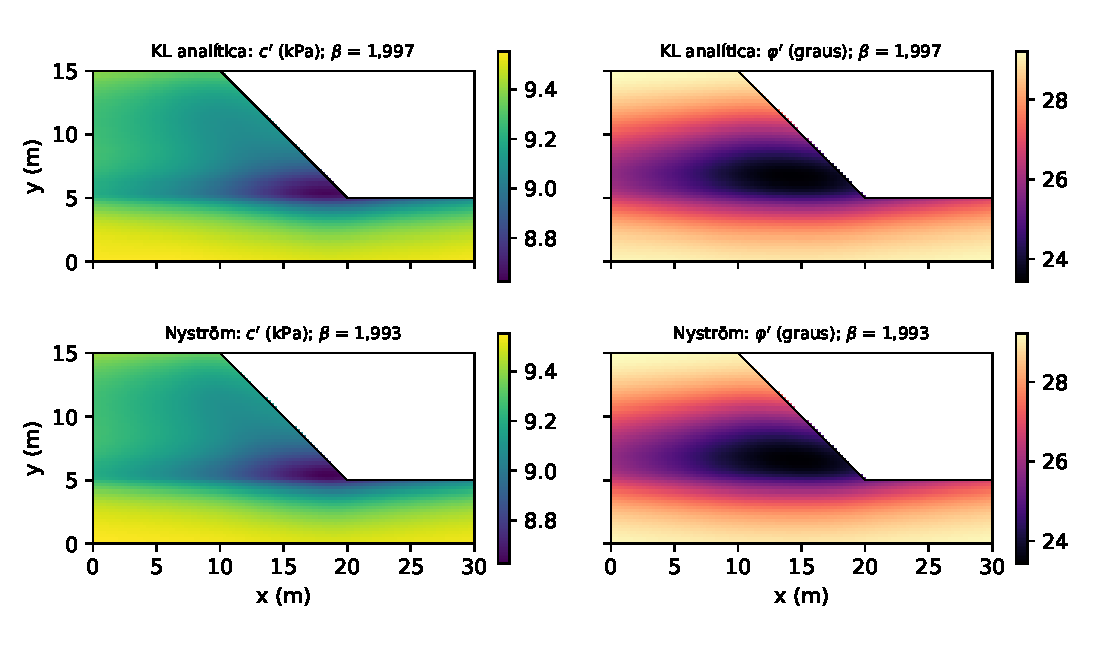
\includegraphics[width=\textwidth]{figs/ponto_projeto.pdf}
\caption{$c'$ e $\varphi'$ no ponto de projeto do FORM modal: KL analítica ($M = 100$, em cima) e Nyström ($M = 200$,
embaixo), com as mesmas escalas de cor.}\label{fig:pp}\end{figure}

\section{O plano de trabalho e a situação}
\begin{table}[H]\centering\small
\resizebox{\ifdim\width>\textwidth\textwidth\else\width\fi}{!}{%
\begin{tabular}{lp{0.55\textwidth}p{0.3\textwidth}}
\toprule
Etapa & O quê & Situação \\
\midrule
0 & Cho2010 no fermi: direto, AI pela banda e pelo FORM & pronta \\
1 & SRM corrigido ($F_0 = 0{,}8$): o antigo contra o novo nas mesmas realizações & pronta \\
2 & FORM ($M = 10$, 20) e AI pelo ponto de projeto; teste linear sem MEF & pronta; sem viés (Seção~\ref{sec:vies}) \\
2b & base de Nyström contra a analítica & o mesmo ponto de projeto (Seção~\ref{sec:form}); AI de Nyström no fermi (fase 4) \\
2c & gradiente do FORM pela projeção modal & validado; a AI modal não tem viés; 10 sementes no fermi (fase 4) \\
3 & $P_f$ pequena ($r = -0{,}7$), tamanho do piloto, custo & pronta, com o direto de 25\,000 (93 falhas) \\
4 & FORM e AI na chuva & o direto de 10\,000 está terminando; falta o código do FORM na chuva \\
5 & investigação da chuva & não começou \\
\bottomrule
\end{tabular}}
\end{table}

\section{Testes e resultados}
\textbf{Cores nas tabelas:} em cada coluna de desempenho, \textcolor{azul}{\textbf{azul}} é o melhor valor e
\textcolor{verm}{\textbf{vermelho}} o pior. CoV e custo: o menor é o melhor; ganho: o maior; dif.: o menor em módulo. Só
entram as AI completas (1000 realizações): o direto é a referência, e as parciais e as da fila ficam de fora. No teste
linear, a comparação é entre as duas direções, linha a linha. Atenção: um $|$dif.$|$ abaixo de 2 é compatível com o
acaso; o azul na dif. não quer dizer que o método é mais exato, e o vermelho só é um sinal quando passa de 2.

\subsection{SRM corrigido (etapa 1)}
Com as mesmas realizações nas duas versões:
\begin{itemize}
  \item \textbf{Cho2010:} as falhas são idênticas (22 e 22 em 1000).
  \item \textbf{Chuva:} 4 realizações passam a falhar e 1 deixa de falhar (McNemar $p = 0{,}38$), cerca de $+0{,}5$ ponto.
\end{itemize}
O efeito é pequeno, e o SRM novo é o correto. As duas versões do programa reproduzem o mesmo FS (diferença de 0,0000), e o
PC reproduz o fermi.
\begin{figure}[H]\centering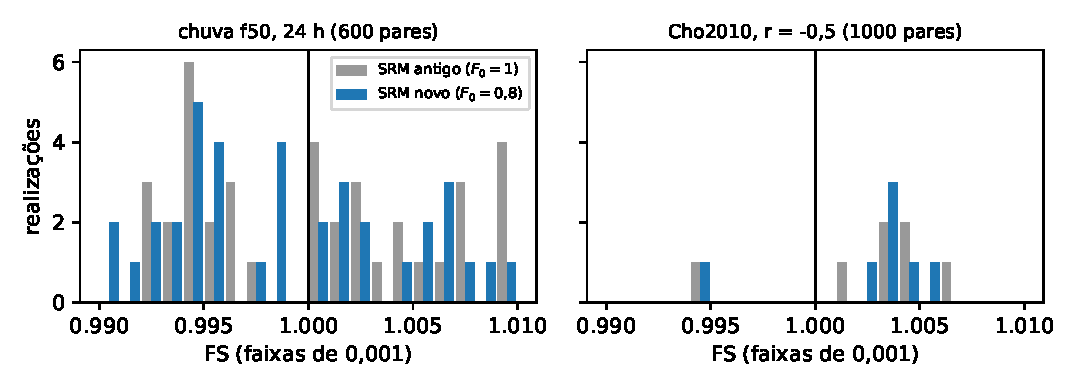
\includegraphics[width=0.9\textwidth]{figs/srm_hist.pdf}\caption{FS perto de 1 nas duas
versões do SRM.}\end{figure}

\subsection{Cho2010, $r = -0{,}5$: AI contra o direto (etapas 0, 2 e 2c)}
\begin{table}[H]\centering\small
\resizebox{\ifdim\width>\textwidth\textwidth\else\width\fi}{!}{%
\begin{tabular}{lrrrrr}
\toprule
Método & $N$ & $P_f$ (\%) & CoV (\%) & dif. (desvios) & ganho \\
\midrule
Monte Carlo direto (fermi) & 24000 & 1{,}70 & 4{,}9 & --- & 1 \\
AI pela banda (entropia cruzada) & 1000 & 1{,}74 & \textcolor{verm}{\textbf{11{,}1}} & \textcolor{azul}{\textbf{0{,}2}} & \textcolor{verm}{\textbf{4{,}6}} \\
AI pelo FORM $M = 10$ & 1000 & 1{,}54 & 8{,}8 & -1{,}0 & 8{,}3 \\
AI pelo FORM $M = 20$ & 1000 & 1{,}53 & 6{,}3 & -1{,}3 & 16{,}2 \\
AI pelo FORM $M = 20$, semente 4 & 1000 & 1{,}72 & 5{,}9 & \textcolor{azul}{\textbf{0{,}2}} & 16{,}3 \\
AI pelo FORM $M = 20$, semente 5 & 1000 & 1{,}90 & 6{,}1 & 1{,}4 & 14{,}1 \\
AI pela banda, piloto na Tri(0) [PC] & 1000 & 1{,}66 & 10{,}8 & \textcolor{azul}{\textbf{-0{,}2}} & 5{,}1 \\
AI pela banda, piloto na Tri(1) [PC] & 1000 & 1{,}89 & 9{,}4 & 1{,}0 & 5{,}9 \\
AI pela banda, piloto na Tri(2) [PC] & 1000 & 1{,}92 & 7{,}8 & 1{,}3 & 8{,}5 \\
AI pelo FORM $M = 100$, direção da Tri(0) [PC] & 1000 & 1{,}36 & 9{,}3 & \textcolor{verm}{\textbf{-2{,}2}} & 8{,}4 \\
AI pelo FORM $M = 100$, gradiente modal [PC] & 1000 & 1{,}57 & 6{,}9 & -0{,}9 & 12{,}9 \\
AI pelo FORM $M = 200$, gradiente modal [PC] & 1000 & 1{,}57 & 6{,}8 & -1{,}0 & 13{,}6 \\
AI pelo FORM $M = 100$ modal, semente 6 [fermi] & 1000 & 1{,}66 & \textcolor{azul}{\textbf{5{,}8}} & -0{,}3 & \textcolor{azul}{\textbf{17{,}6}} \\
AI pelo FORM $M = 200$ modal, semente 7 [fermi] & 1000 & 1{,}78 & 5{,}9 & 0{,}6 & 15{,}6 \\
AI pela banda, piloto Tri(1), semente 10 [fermi] & 1000 & 1{,}79 & 10{,}3 & 0{,}4 & 5{,}2 \\
\bottomrule
\end{tabular}}
\caption{$r = -0{,}5$ (Cho: $P_f = 1{,}71\,\%$). O direto terminou: 24\,000 realizações. ``dif.'' é a diferença AI
$-$ direto em desvios. Sem indicação, o FORM usa a semente 3 e a banda a semente 1; [PC] e [fermi] dizem onde rodou.}
\end{table}
\begin{figure}[H]\centering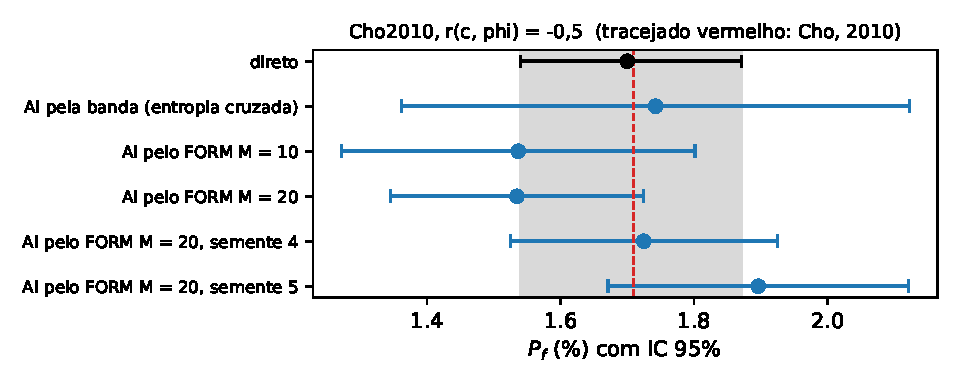
\includegraphics[width=0.75\textwidth]{figs/pf_r05.pdf}\caption{$P_f$ e IC 95\,\%, $r = -0{,}5$.}\end{figure}

\subsection{$P_f$ pequena, $r = -0{,}7$ (etapa 3)}
\begin{table}[H]\centering\small
\resizebox{\ifdim\width>\textwidth\textwidth\else\width\fi}{!}{%
\begin{tabular}{lrrrrr}
\toprule
Método & $N$ & $P_f$ (\%) & CoV (\%) & dif. (desvios) & ganho \\
\midrule
Monte Carlo direto (fermi) & 25000 & 0{,}37 & 10{,}4 & --- & 1 \\
AI pela banda (entropia cruzada) & 1000 & 0{,}45 & 16{,}3 & 0{,}9 & 8{,}4 \\
AI pelo FORM $M = 10$ & 1000 & 0{,}31 & 11{,}6 & \textcolor{verm}{\textbf{-1{,}1}} & 23{,}5 \\
AI pelo FORM $M = 20$ & 1000 & 0{,}35 & 8{,}6 & -0{,}4 & 38{,}3 \\
AI pelo FORM $M = 20$, semente 4 & 1000 & 0{,}35 & \textcolor{azul}{\textbf{7{,}4}} & -0{,}4 & \textcolor{azul}{\textbf{51{,}1}} \\
AI pelo FORM $M = 20$, semente 5 & 1000 & 0{,}38 & 8{,}4 & \textcolor{azul}{\textbf{0{,}2}} & 36{,}9 \\
AI pela banda, semente 4 & 1000 & 0{,}40 & \textcolor{verm}{\textbf{24{,}6}} & 0{,}3 & \textcolor{verm}{\textbf{4{,}1}} \\
\bottomrule
\end{tabular}}
\caption{$r = -0{,}7$ (Cho: $P_f \approx 0{,}4\,\%$).}
\end{table}

\subsection{A semente 3 e as repetições independentes}
As primeiras AI pelo FORM usavam todas a semente 3 (números aleatórios comuns): com pontos de projeto quase iguais, elas dão
quase a mesma estimativa e não são independentes. As repetições com as sementes 4 e 5 (FORM $M = 20$) e 6 e 7 (FORM
modal, $M = 100$ e 200) separam o acaso do viés:
\begin{table}[H]\centering\small
\resizebox{\ifdim\width>\textwidth\textwidth\else\width\fi}{!}{%
\begin{tabular}{lrrrrr}
\toprule
Caso & sementes & $P_f$ de cada (\%) & média (\%) & direto (\%) & dif. (desvios) \\
\midrule
$r = -0{,}5$, FORM $M = 20$ & 3 & 1{,}53, 1{,}72, 1{,}90 & 1{,}72 & 1{,}70 & 0{,}2 \\
$r = -0{,}5$, FORM $M = 20$, 100 e 200 modal & 5 & 1{,}53, 1{,}72, 1{,}90, 1{,}66, 1{,}78 & 1{,}72 & 1{,}70 & 0{,}2 \\
$r = -0{,}7$, FORM $M = 20$ & 3 & 0{,}35, 0{,}35, 0{,}38 & 0{,}36 & 0{,}37 & -0{,}3 \\
\bottomrule
\end{tabular}}
\caption{AI pelo FORM com sementes independentes, 1000 realizações cada. A dif. usa o desvio da média,
$\sqrt{\sum s_i^2}/k$, e o do direto.}
\end{table}

\subsection{A AI pelo FORM tem viés? O teste com o próprio direto (KL e Nyström)}\label{sec:vies}
Com a semente 3, todas as AI pelo FORM ficaram abaixo do direto (1,53 a 1,57\,\% contra 1,70\,\%), e a AI modal, a mais
eficiente, parecia convergir para o valor errado. Uma AI com deslocamento fixo não tem viés, mas pode se comportar como se
tivesse. Se a densidade de amostragem quase não visita uma parte da região de falha (outro modo de ruptura, longe do
ponto de projeto), a estimativa sai quase sempre baixa, e o CoV estimado fica menor que o verdadeiro. O direto permite
testar isso sem nenhuma análise nova (\path{Projects/Cho2010/diagnostico_ai.py}):
\begin{enumerate}
  \item \textbf{Os $\bm\xi$ de cada realização} saem de uma cópia do gerador do \texttt{RandomField} em Python
    (xoshiro256** e Box--Muller, uma semente por realização e campo). A cópia confere com o peso de cada amostra de cada
    AI (erro $\le 5\times10^{-9}$). Junto com a KL analítica em Python, ela
    também confere com o campo que o programa grava (diferença $\le 5\times10^{-6}$, a precisão do CSV).
  \item \textbf{Modo de ruptura fora da AI.} As 408 falhas do direto, projetadas na direção
    do ponto de projeto ($t = \bm\alpha\cdot\bm\xi$), ficam todas onde a AI amostra (Figura~\ref{fig:vies_t}). Na direção
    modal, o menor $t$ é 0{,}80, e só 3 falhas ficam abaixo de
    1,5. A variância verdadeira de cada AI sai do direto pela identidade $E_h[I w^2] = E_\varphi[I w]$, com as falhas do
    direto, e é a que a AI estima (``CoV verd.'' na Tabela~\ref{tab:vies05}): 6{,}2\,\% contra 6{,}9\,\% no modal $M = 100$. Só a direção errada da Tri(0)
    subestima o próprio CoV (9{,}3\,\% estimado contra 12{,}3\,\% verdadeiro): o $-2{,}2$ desvio da Tabela~1 vinha daí.
  \item \textbf{Base de Nyström.} Com $T$ (Seção~\ref{sec:kl}), as realizações do direto vão para as coordenadas de
    Nyström, e o mesmo teste vale para as AI de Nyström: $t \ge 0{,}91$, e
    CoV verdadeiro de 6{,}1 a 6{,}3\,\%, contra 6{,}0 a 6{,}2\,\% estimados. Os FS são os do campo
    analítico, uma aproximação: o campo de Nyström é a projeção dele. A regressão de $\ln\mathrm{FS}$ explica o mesmo nas
    duas bases ($R^2 = 0{,}965$ e $0{,}965$).
  \item \textbf{A sorte de cada amostra.} A variável de controle mede a sorte de cada amostra no que a regressão explica.
    A amostra da semente 3 é azarada: o controle fica em 98\,\% da sua média exata na
    AI modal, 96\,\% no FORM $M = 20$ e 95\,\%
    no Nyström $M = 200$. Corrigida, a AI modal da semente 3 vai de 1{,}57 para 1{,}60\,\%. O direto corrigido fica em 1{,}705 $\pm$ 0{,}040\,\%
    (CoV de 2{,}4\,\%), o equivalente a 104\,015 realizações.
\end{enumerate}
\begin{figure}[H]\centering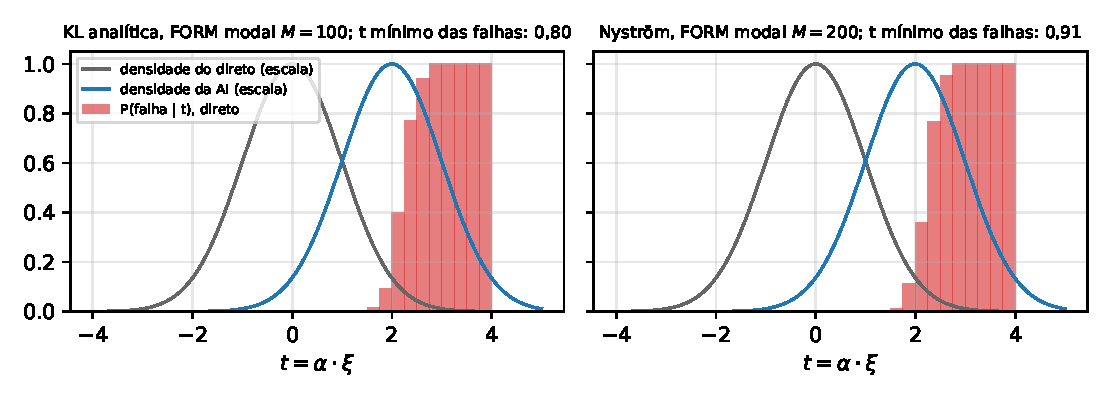
\includegraphics[width=\textwidth]{figs/vies_t.pdf}
\caption{A chance de falha do direto em cada faixa de $t = \bm\alpha\cdot\bm\xi$ (barras) e as densidades de $t$ no
direto e na AI (curvas, em escala). A AI amostra toda a região onde o direto falha.}\label{fig:vies_t}\end{figure}
\begin{table}[H]\centering\small
\resizebox{\ifdim\width>\textwidth\textwidth\else\width\fi}{!}{%
\begin{tabular}{llrrrrrrrr}
\toprule
AI & base & semente & $N$ & $P_f$ (\%) & CoV (\%) & CoV verd. (\%) & $t_{\min}$ & $P_f$ corr. (\%) & CoV corr. (\%) \\
\midrule
Monte Carlo direto & --- & 2010 & 24000 & 1{,}70 & 4{,}9 & --- & --- & 1{,}71 & 2{,}4 \\
FORM $M = 10$, dif. centrais & KL & 3 & 1000 & 1{,}54 & 8{,}8 & 7{,}8 & 0{,}62 & 1{,}66 & 4{,}5 \\
FORM $M = 20$, dif. centrais & KL & 3 & 1000 & 1{,}53 & 6{,}3 & 5{,}9 & 1{,}31 & 1{,}60 & 4{,}3 \\
FORM $M = 20$, dif. centrais & KL & 4 & 1000 & 1{,}72 & 5{,}9 & 5{,}9 & 1{,}31 & 1{,}64 & 4{,}2 \\
FORM $M = 20$, dif. centrais & KL & 5 & 1000 & 1{,}90 & 6{,}1 & 5{,}9 & 1{,}31 & 1{,}76 & 4{,}6 \\
FORM modal $M = 100$ & KL & 3 & 1000 & 1{,}57 & 6{,}9 & 6{,}2 & 0{,}80 & 1{,}60 & 5{,}1 \\
FORM modal $M = 200$ & KL & 3 & 1000 & 1{,}57 & 6{,}8 & 6{,}0 & 0{,}93 & 1{,}60 & 5{,}0 \\
FORM modal $M = 200$, campo de 200 termos & KL & 3 & 1000 & 1{,}56 & 6{,}8 & 6{,}0 & 0{,}93 & 1{,}59 & 5{,}0 \\
FORM modal $M = 100$ & KL & 6 & 1000 & 1{,}66 & \textcolor{azul}{\textbf{5{,}8}} & 6{,}2 & 0{,}80 & 1{,}65 & 4{,}1 \\
FORM modal $M = 200$ & KL & 7 & 1000 & 1{,}78 & 5{,}9 & 6{,}0 & 0{,}93 & 1{,}75 & 4{,}6 \\
direção da Tri(0), $M = 100$ & KL & 3 & 1000 & 1{,}36 & \textcolor{verm}{\textbf{9{,}3}} & 12{,}3 & 0{,}58 & 1{,}57 & \textcolor{verm}{\textbf{5{,}4}} \\
FORM modal $M = 20$ & Nyström & 3 & 1000 & 1{,}57 & 6{,}2 & 6{,}3 & 1{,}02 & 1{,}62 & \textcolor{azul}{\textbf{3{,}8}} \\
FORM modal $M = 200$ & Nyström & 3 & 1000 & 1{,}53 & 6{,}0 & 6{,}1 & 0{,}91 & 1{,}60 & 4{,}0 \\
\bottomrule
\end{tabular}}
\caption{$r = -0{,}5$: as AI pelo ponto de projeto. ``CoV verd.'' é o CoV verdadeiro de cada AI, calculado pelas falhas
do direto; $t_{\min}$ é o menor $t$ entre as falhas do direto; ``corr.'' é a estimativa com a variável de controle.
Em Nyström, o direto vai para a base de Nyström pela mudança de base.}\label{tab:vies05}
\end{table}
\begin{table}[H]\centering\small
\resizebox{\ifdim\width>\textwidth\textwidth\else\width\fi}{!}{%
\begin{tabular}{lrrrrrr}
\toprule
Grupo & sementes & $P_f$ média (\%) & dif. & $P_f$ corr. média (\%) & dif. & desvio entre sementes / estimado \\
\midrule
$r = -0{,}5$, KL (modal; $M = 20$ em s4 e s5) & 5 & 1{,}728 $\pm$ 0{,}047 & $0{,}3$ & 1{,}679 $\pm$ 0{,}034 & $-0{,}5$ & 0{,}122 / 0{,}106 \\
$r = -0{,}5$, Nyström (modal) & 1 & 1{,}527 $\pm$ 0{,}092 & $-1{,}4$ & 1{,}600 $\pm$ 0{,}064 & $-1{,}4$ & --- \\
$r = -0{,}7$, KL ($M = 20$) & 3 & 0{,}361 $\pm$ 0{,}017 & $-0{,}3$ & 0{,}350 $\pm$ 0{,}015 & $-1{,}0$ & 0{,}016 / 0{,}030 \\
\bottomrule
\end{tabular}}
\caption{As sementes independentes (uma AI por semente; a 3 é a do PC). A dif. é a diferença para o direto, em desvios;
a corrigida usa o direto corrigido. A última coluna compara a dispersão real entre as sementes com o desvio que cada AI
estima.}\label{tab:sementes}
\end{table}
\begin{figure}[H]\centering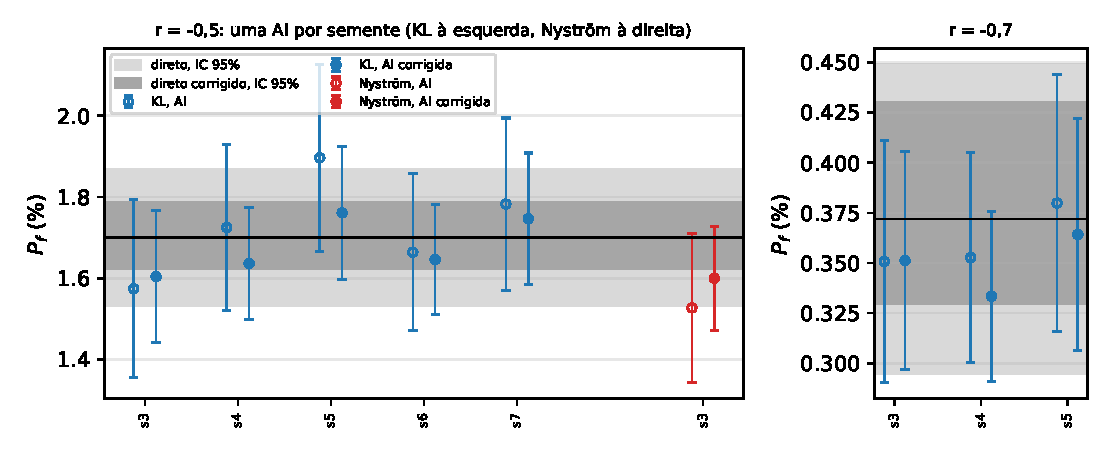
\includegraphics[width=\textwidth]{figs/vies_sementes.pdf}
\caption{Uma AI por semente, com IC 95\,\%: vazado, a estimativa da AI; cheio, a corrigida. As faixas são o IC 95\,\% do
direto (claro) e do direto corrigido (escuro).}\label{fig:vies_sementes}\end{figure}
\textbf{$r = -0{,}7$} (direto de 25\,000, 93
falhas): $t \ge 2{,}20$ na direção do FORM $M = 20$ (1{,}23
no $M = 10$). O CoV verdadeiro é 7{,}6\,\%, e as AI estimam de 7{,}4 a 8{,}6\,\%.
As sementes 3, 4 e 5, corrigidas, dão 0{,}351, 0{,}333, 0{,}364\,\%, contra 0{,}380 $\pm$ 0{,}025\,\% do direto corrigido ($-1{,}0$ desvio).
\begin{table}[H]\centering\small
\resizebox{\ifdim\width>\textwidth\textwidth\else\width\fi}{!}{%
\begin{tabular}{llrrrrrrrr}
\toprule
AI & base & semente & $N$ & $P_f$ (\%) & CoV (\%) & CoV verd. (\%) & $t_{\min}$ & $P_f$ corr. (\%) & CoV corr. (\%) \\
\midrule
Monte Carlo direto & --- & 2010 & 25000 & 0{,}372 & 10{,}4 & --- & --- & 0{,}380 & 6{,}6 \\
FORM $M = 10$, dif. centrais & KL & 3 & 1000 & 0{,}313 & \textcolor{verm}{\textbf{11{,}6}} & 12{,}2 & 1{,}23 & 0{,}324 & \textcolor{verm}{\textbf{9{,}3}} \\
FORM $M = 20$, dif. centrais & KL & 3 & 1000 & 0{,}351 & 8{,}6 & 7{,}6 & 2{,}20 & 0{,}351 & 7{,}8 \\
FORM $M = 20$, dif. centrais & KL & 4 & 1000 & 0{,}353 & \textcolor{azul}{\textbf{7{,}4}} & 7{,}6 & 2{,}20 & 0{,}333 & \textcolor{azul}{\textbf{6{,}3}} \\
FORM $M = 20$, dif. centrais & KL & 5 & 1000 & 0{,}380 & 8{,}4 & 7{,}6 & 2{,}20 & 0{,}364 & 7{,}9 \\
\bottomrule
\end{tabular}}
\caption{$r = -0{,}7$: as AI pelo ponto de projeto, como na Tabela~\ref{tab:vies05}.}\label{tab:vies07}
\end{table}
\textbf{Conclusão.}
\begin{itemize}
  \item Nenhum modo de ruptura fica fora da AI, e a variância verdadeira é a estimada.
  \item As sementes independentes acertam o direto, nas duas bases. A semente 3 é uma tiragem baixa, comum a todas as
    AI que a usam.
  \item As repetições da fase 4 no fermi fecham a questão: 10 sementes do FORM modal analítico e 10 do de Nyström, com as
    mesmas sementes nas duas bases. Elas dão a distribuição do estimador.
  \item A variável de controle é um ganho à parte, sem custo: de 1{,}7 a 3{,}2 vezes menos realizações nas AI e 4{,}3 no direto.
\end{itemize}

\subsection{Comparação das bases com a mesma variância}
A variância do campo nos pontos do talude depende da base e de $M$ (\path{runs/cho2010/nystrom/variancia_bases.py}):
\begin{table}[H]\centering\small
\resizebox{\ifdim\width>\textwidth\textwidth\else\width\fi}{!}{%
\begin{tabular}{rrr}
\toprule
$M$ & analítica (retângulo) & Nyström (talude) \\
\midrule
10 & 0,60 & 0,65 \\
20 & 0,72 & 0,76 \\
50 & 0,84 & 0,86 \\
100 & 0,90 & 0,90 \\
200 & 0,935 & 0,931 \\
400 & 0,96 & 0,94 \\
2000 & 0,99 & 0,95 (teto) \\
\bottomrule
\end{tabular}}
\caption{Variância média do campo nos pontos do talude (alvo 1). O teto de Nyström vem da quadratura de 2400 nós: a
interpolação entre os nós não reproduz o bico do kernel exponencial.}
\end{table}
Com poucos termos, Nyström retém mais variância; em $M \approx 200$ as duas se igualam (≈0,93). A AI analítica usa 2000
termos (0,99), e a de Nyström 200 (0,93): são modelos de campo diferentes. Mas a variância que falta está nos modos
altos, que quase não mudam o FS (a média ao longo da banda de ruptura os filtra): o $\beta$ do FORM vai de 2,001
($M = 100$) para 1,999 ($M = 200$). Por isso a $P_f$ do campo com 0,93 deve ficar perto da do campo completo; a
estimativa inicial, de 1,3 a 1,4\,\% pela variância, estava errada. A comparação justa das bases usa os dois campos
com a mesma variância:
\begin{table}[H]\centering\small
\resizebox{\ifdim\width>\textwidth\textwidth\else\width\fi}{!}{%
\begin{tabular}{lrrr}
\toprule
Campo (variância ≈0,93) & $N$ & $P_f$ (\%) & CoV (\%) \\
\midrule
Nyström, 200 termos (ponto do FORM modal Nyström $M = 200$) & 1000 & 1{,}53 & \textcolor{azul}{\textbf{6{,}0}} \\
Nyström, 200 termos (ponto do FORM modal Nyström $M = 20$) & 1000 & 1{,}57 & 6{,}2 \\
analítica truncada em 200 termos (ponto do FORM modal $M = 200$) & 1000 & 1{,}56 & \textcolor{verm}{\textbf{6{,}8}} \\
\bottomrule
\end{tabular}}
\caption{AI no PC, semente 3, a mesma das AI analíticas da Tabela 1 (os sorteios são os mesmos). A referência de
24\,000 é do campo completo (2000 termos) e só vale aproximadamente aqui.}
\end{table}

\subsection{O piso do SRM em $F_0 = 0{,}8$}
Nenhuma realização das AI deu FS abaixo de 0,8 (o mínimo foi 0,802). É o mesmo mecanismo do buraco em $F = 1$: um talude
com FS verdadeiro logo abaixo de $F_0$ às vezes converge o peso com $F_0$ e devolve $\approx F_0$. Para a $P_f$ não muda
nada (o FS continua $< 1$), mas a cauda inferior do FS fica distorcida (≈1 realização em 1000). Correção proposta:
recomeçar de $F_0/2$ quando o caminho de $F$ colapsa logo no início.

\subsection{Custo total para CoV$(P_f) = 10\,\%$}
\begin{table}[H]\centering\small
\resizebox{\ifdim\width>\textwidth\textwidth\else\width\fi}{!}{%
\begin{tabular}{lrr}
\toprule
Método & $r = -0{,}5$ & $r = -0{,}7$ \\
\midrule
Monte Carlo direto & 5782 & 26782 \\
AI pela banda (entropia cruzada) & \textcolor{verm}{\textbf{2238}} & \textcolor{verm}{\textbf{3645}} \\
AI pelo FORM $M = 10$ & 896 & 1518 \\
AI pelo FORM $M = 20$ & \textcolor{azul}{\textbf{639}} & \textcolor{azul}{\textbf{984}} \\
\bottomrule
\end{tabular}}
\caption{Análises de elementos finitos, com o piloto (1000) e o FORM incluídos. Com o piloto na malha grossa (custo
1/20, Seção~\ref{sec:hip}), a AI pela banda cai para ≈1300 e ≈2700.}
\end{table}

\subsection{O teste linear (sem elementos finitos)}
\begin{table}[H]\centering\small
\resizebox{\ifdim\width>\textwidth\textwidth\else\width\fi}{!}{%
\begin{tabular}{rrrrr}
\toprule
$\beta$ & $P_f$ exata & direto ($10^6$) & AI na direção exata & AI a 17{,}6$^\circ$ da direção \\
\midrule
2 & 2.275e-02 & 2{,}27\,\% & \textcolor{azul}{\textbf{0{,}8\,\% (0{,}5)}} & \textcolor{verm}{\textbf{-2{,}9\,\% (-1{,}6)}} \\
3 & 1.350e-03 & 0{,}13\,\% & \textcolor{azul}{\textbf{0{,}9\,\% (0{,}5)}} & \textcolor{verm}{\textbf{-4{,}7\,\% (-1{,}7)}} \\
4 & 3.167e-05 & --- & \textcolor{azul}{\textbf{1{,}0\,\% (0{,}4)}} & \textcolor{verm}{\textbf{-9{,}1\,\% (-2{,}6)}} \\
\bottomrule
\end{tabular}}
\caption{Falha $\bm\alpha\cdot\bm\xi > \beta$, com $P_f$ exata. Erro relativo, com o erro em desvios entre parênteses.}
\end{table}
Com o deslocamento na direção exata, a AI acerta até $3\times10^{-5}$. Com a direção um pouco errada, ela sai baixa, e
mais baixa quando $\beta$ cresce.

\subsection{FORM: gradiente modal e as duas bases (etapas 2b e 2c)}\label{sec:nystrom}
\begin{itemize}
  \item \textbf{Validação do gradiente modal} nos pontos de projeto do fermi: ele fica a 9,6$^\circ$ ($M = 10$) e
    8,9$^\circ$ ($M = 20$) do gradiente das diferenças centrais, e o termo dominante ($\varphi'_0$) bate a menos de 4\,\%.
\end{itemize}
\begin{table}[H]\centering\small
\resizebox{\ifdim\width>\textwidth\textwidth\else\width\fi}{!}{%
\begin{tabular}{rrrrr}
\toprule
$M$ & variância retida (Nyström) & $\beta$ analítica & $\beta$ Nyström & análises por FORM \\
\midrule
10 & 0{,}655 & 2{,}151 & 2{,}062 & 4 \\
20 & 0{,}769 & 2{,}040 & 2{,}020 & 3 \\
50 & 0{,}876 & 2{,}009 & 2{,}009 & 3 \\
100 & 0{,}933 & 2{,}001 & 2{,}002 & 3 \\
200 & 0{,}970 & 1{,}999 & 1{,}999 & 3 \\
\bottomrule
\end{tabular}}
\caption{$\beta$ do FORM com o gradiente modal na malha usual. Com diferenças centrais: 2,115 ($M = 10$, 123 análises) e
2,012 ($M = 20$, 243).}
\end{table}
\begin{figure}[H]\centering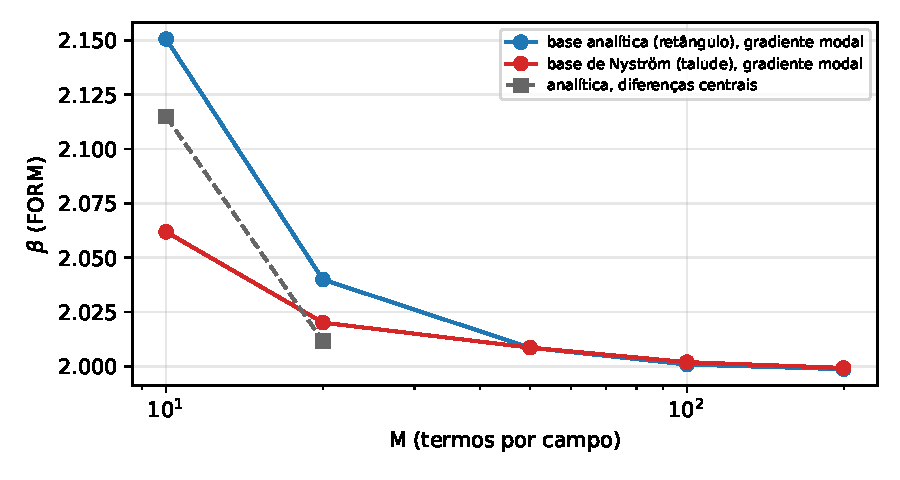
\includegraphics[width=0.6\textwidth]{figs/beta_M.pdf}\caption{$\beta(M)$: a base de
Nyström converge com menos termos.}\end{figure}
A base de Nyström chega mais perto do $\beta$ convergido com poucos termos ($M = 10$: 2,062 contra 2,151), e as duas
coincidem a partir de $M = 50$. É o mesmo efeito da placa curva do \path{relatorio_kl_form}. O $\beta$ converge para
$\approx 2{,}00$, mas a $P_f$ do FORM sozinho ($\approx 2{,}3\,\%$) superestima a do direto em ≈30\,\%: é o erro de
linearizar uma superfície de falha curva. Por isso o FORM entra só como deslocamento da AI.

\subsection{A referência da chuva (etapa 4)}
\begin{table}[H]\centering\small
\resizebox{\ifdim\width>\textwidth\textwidth\else\width\fi}{!}{%
\begin{tabular}{lrrrrr}
\toprule
Método & $N$ & $P_f$ (\%) & CoV (\%) & dif. (desvios) & ganho \\
\midrule
Monte Carlo direto (fermi) & 9093 & 5{,}45 & 4{,}4 & --- & 1 \\
AI pela banda, semente 1 & 1000 & 6{,}18 & \textcolor{azul}{\textbf{7{,}0}} & \textcolor{verm}{\textbf{1{,}5}} & \textcolor{azul}{\textbf{3{,}1}} \\
AI pela banda, semente 2 & 1000 & 5{,}74 & \textcolor{verm}{\textbf{8{,}2}} & \textcolor{azul}{\textbf{0{,}5}} & \textcolor{verm}{\textbf{2{,}4}} \\
\bottomrule
\end{tabular}}
\caption{f50 a 31,05\,mm/h, FS em 24\,h.}
\end{table}

\section{Hipóteses}\label{sec:hip}
\subsection*{Confirmadas}
\begin{itemize}
  \item A AI não tem viés com qualquer deslocamento fixado antes; o deslocamento só muda a variância (teste linear e Ceron).
  \item O SRM antigo tinha um buraco logo abaixo de FS = 1; o efeito na $P_f$ é pequeno.
  \item \textbf{Há um só modo de ruptura} no Cho2010, nas duas bases: todas as falhas do direto ficam onde a AI pelo
    FORM amostra ($t = \bm\alpha\cdot\bm\xi \ge 0{,}80$ na direção modal, com só
    3 das 408 abaixo de 1,5;
    $t \ge 2{,}20$ com $r = -0{,}7$), e a variância verdadeira da AI,
    calculada pelas falhas do direto, é a que a AI estima (Seção~\ref{sec:vies}). A banda de ruptura das falhas é a mesma
    no direto e na AI.
  \item \textbf{O ponto de projeto é o mesmo nas duas bases:} levado para as coordenadas de Nyström, o ponto analítico
    fica a 3{,}2$^\circ$ do de Nyström, e os campos de $\varphi'$ diferem em
    menos de 0,1$^\circ$ (Figura~\ref{fig:pp}).
  \item \textbf{A variável de controle dá um ganho extra sem custo:} de 1{,}7 a
    3{,}2 nas AI de $r = -0{,}5$ e 4{,}3
    no direto, cuja referência vai a 1{,}705 $\pm$ 0{,}040\,\%.
  \item \textbf{O piloto pode ser pequeno:} com 250 realizações, o deslocamento da banda custa só ≈5\,\% de variância.
  \item \textbf{O piloto pode rodar em malha grossa:} o elite é escolhido por ordem, e a ordem das realizações quase não
    muda. Com o piloto na Tri(0) (300 vezes mais barata), a AI pela banda acertou o direto ($-0{,}2$ desvio), com o mesmo
    CoV do piloto na malha usual. Tri(1) e Tri(2) também estão nas tabelas.
  \item \textbf{O gradiente modal dá a direção do FORM com 1 análise,} a menos de ≈9$^\circ$ das diferenças centrais, e o
    FORM converge em 3 análises.
  \item \textbf{A base de Nyström precisa de menos termos} que a analítica para o mesmo $\beta$.
  \item \textbf{A AI pelo FORM não tem viés} ($r = -0{,}5$), nas duas bases (Seção~\ref{sec:vies}). Com a semente 3, as AI saem todas em ≈1,55\,\% (os sorteios são os mesmos). As 5 sementes independentes da KL dão, em média, 1{,}728\,\% contra 1{,}700\,\% do direto e, com a variável de controle, 1{,}679 $\pm$ 0{,}034\,\% contra 1{,}705 $\pm$ 0{,}040\,\% ($-0{,}5$ desvio). A direção errada da Tri(0) é a única que subestima o próprio CoV (9{,}3 contra 12{,}3\,\%); com o CoV verdadeiro, o seu desvio cai de $-2{,}2$ para $-1{,}5$.
  \item \textbf{A AI pelo FORM com $r = -0{,}7$ também não tem viés detectável:} as sementes 3, 4 e 5, corrigidas, dão 0{,}351, 0{,}333, 0{,}364\,\%, contra 0{,}380 $\pm$ 0{,}025\,\% do direto corrigido (25\,000 realizações, 93 falhas): $-1{,}0$ desvio.
\end{itemize}
\subsection*{Descartadas}
\begin{itemize}
  \item \textbf{O FORM na malha Tri(0)} (76 equações, FS 1,47 contra 1,20): $\beta = 4{,}08$ e direção a 31,7$^\circ$ da
    certa. O erro da malha desloca o ponto de projeto, e não só o FS. Com a direção da Tri(0) e a distância da malha usual
    ($\beta = 2{,}32$), a AI funciona, mas pior que o FORM na malha usual.
\end{itemize}
\subsection*{Sob investigação}
\begin{itemize}
  \item \textbf{O campo de $k$ na chuva:} o gradiente modal pega $c'$ e $\varphi'$; o $k$ age pelo transiente e
    precisaria do adjunto. Hoje o $k$ pesa pouco na chuva f50 ($\alpha^2_k \approx 0$), e a AI continua sem viés sem
    deslocá-lo.
\end{itemize}

\section{Próximos passos}
\begin{enumerate}
  \item \textbf{Fase 4 no fermi} (≈7\,h): 10 sementes do FORM modal analítico e 10 do de Nyström, as mesmas nas duas
    bases. Dão a distribuição do estimador e fecham a questão do viés (Seção~\ref{sec:vies}).
  \item \textbf{Etapa 4:} o FORM com gradiente modal e a AI pelo ponto de projeto na chuva, contra o direto de 10\,000
    (terminando no fermi).
  \item \textbf{Variável de controle} nas AI pela banda e na chuva. Para o artigo da AI: o ganho contra o custo total
    (FORM, piloto e controle), de $P_f \approx 2\,\%$ a $0{,}4\,\%$.
  \item \textbf{Arquivamento dos documentos:} a formulação separada dos resultados, com um índice único (proposta em
    discussão).
\end{enumerate}

\section{Mapa dos relatórios}\label{sec:mapa}
Os documentos estão espalhados; esta lista diz onde está cada um e o que tem. Os caminhos relativos são a partir de
\path{~/projects/neopz-master}.

\begin{longtable}{p{0.40\textwidth}p{0.55\textwidth}}
\toprule
Documento & O que tem \\
\midrule
\endhead
\multicolumn{2}{l}{\textbf{Formulação e modelo}} \\
\path{docs/biot_nao_saturado/biot_nao_saturado_agua_ar5.pdf} & formulação poroelástica não saturada (esqueleto, água e ar), a implementação no NeoPZ, Rahardjo et al. (2007), benchmarks (49 p.) \\
\path{~/Dropbox/UnsaturatedSoil/formulacao/formulacao/formulacao.pdf} & formulação acoplada $u$--$p_w$--$p_a$ com Mohr--Coulomb associado: discretização, resíduos e jacobiano (25 p.) \\
\path{~/Dropbox/UnsaturatedSoil/formulacao/formulacao/resumo_nao_saturado.pdf} & resumo da formulação $u$--$p_w$--$p_a$ (13 p.) \\
\path{docs/slope_mohr_coulomb/relatorio.pdf} & talude Mohr--Coulomb no NeoPZ: correções da plasticidade, FS e rebaixamento (18 p.) \\
\path{docs/slope_mohr_coulomb/nota_uqp.pdf} & nota: formulação de três campos $u$--$q$--$p$ (6 p.) \\
\path{docs/fs_arc_length/relatorio_fs.pdf} & FS de talude não saturado sob chuva: SRM e GIM com e sem arc-length, sensibilidade e parâmetros (34 p.) \\
\multicolumn{2}{l}{\textbf{Campos aleatórios, FORM e amostragem por importância}} \\
\path{~/relatorio_kl_form/relatorio.pdf} & estudo do Ghanem \& Spanos: KL analítica, Nyström e Galerkin, MC e FORM nas placas (quadrada e curva) \\
\path{Projects/SlopeRandomFieldRefinement/relatorio/implementacao_form_ai.pdf} & como o FORM e a AI foram implementados no NeoPZ (5 p.) \\
\path{Projects/Cho2010/nystrom_ai/ai_nystrom.pdf} & AI com a KL de Nyström, um roteiro testado em Mathematica (5 p.) \\
\path{Projects/Confiabilidade/doc/confiabilidade.pdf} & FORM, Monte Carlo e AI em variáveis; talude infinito \\
\path{Projects/GuiaEstudo/guia_estudo.pdf} & guia de estudo que liga tudo (inclui o FORM com a base da KL, Eq.~14) \\
\multicolumn{2}{l}{\textbf{Resultados das campanhas}} \\
\path{Projects/SlopeRandomFieldRefinement/relatorio/relatorio_chuva.pdf} & Monte Carlo da chuva (Rahardjo), Seção 7: AI \\
\path{Projects/SlopeRandomFieldRefinement/relatorio/relatorio_rebaixamento.pdf} & rebaixamento do Ceron, Monte Carlo direto e AI (validação 15,70\,\% contra 15,87\,\%) \\
\path{Projects/SlopeRandomFieldRefinement/relatorio/relatorio_solos.pdf} & os três solos do Rahardjo sob chuva \\
\path{Projects/PlanoDeTrabalho/README.md} & o plano de trabalho (etapas 0 a 5, 2b e 2c) \\
\path{Projects/PlanoDeTrabalho/ETAPA0/relatorio_etapa0.pdf} & etapa 0: a AI da chuva no fermi e a prévia do Cho2010 (SRM antigo; superado pelo das etapas 1 a 3) \\
\path{Projects/PlanoDeTrabalho/ETAPAS1a3/relatorio_etapas.pdf} & etapas 1 a 3: SRM corrigido, FORM e AI, $P_f$ pequena, teste linear, piloto, custo \\
\path{docs/confiabilidade_campos/relatorio_parcial.pdf} & \textbf{este}: o consolidado \\
\bottomrule
\end{longtable}

\end{document}
